% =====================================================================
%  Project report -- SIT Hyderabad template
%  Union-Find Connected Component Labeling for Volumetric Medical Scans
%  Build: pdflatex main.tex (twice, for the page header/links), no BibTeX needed.
%  Upload this folder to Overleaf as-is: main.tex, sit_logo.png, figures/
% =====================================================================
\documentclass[11pt,a4paper]{article}

% ---------------------------------------------------------------------
%  EDIT THE DETAILS BELOW (cover page and acknowledgement)
% ---------------------------------------------------------------------
\newcommand{\AuthorOne}{Tanishq Singh Sisodiya}
\newcommand{\BranchOne}{CSE}
\newcommand{\PRNOne}{25070721054}
\newcommand{\AuthorTwo}{Subhanan Chatterjee}
\newcommand{\BranchTwo}{CSE}
\newcommand{\PRNTwo}{25070721052}
\newcommand{\SubjectName}{Data Structures in C}
\newcommand{\GuideName}{[Project Guide Name]}
\newcommand{\DirectorName}{Dr.\ Rajinikanth Aluvalu}
\newcommand{\ReportDate}{November 2026}
% ---------------------------------------------------------------------

\usepackage[T1]{fontenc}
\usepackage[utf8]{inputenc}
\usepackage{mathptmx}
\usepackage{courier}
\usepackage{microtype}
\usepackage[a4paper,left=1.75cm,right=1.75cm,top=4.37cm,bottom=2.65cm,
            headheight=12pt,headsep=0pt,footskip=10pt]{geometry}
\usepackage{amsmath,amssymb}
\usepackage{graphicx}
\usepackage[table]{xcolor}
\usepackage{booktabs}
\usepackage{array}
\usepackage{tabularx}
\usepackage{enumitem}
\usepackage{placeins}
\usepackage{tikz}
\usepackage{fancyhdr}
\usepackage{lastpage}
\usepackage{titlesec}
\usepackage{listings}
\usepackage[font=small,labelfont={bf,color=sitred},labelsep=period,
            justification=justified,singlelinecheck=false,skip=5pt]{caption}
\usepackage[colorlinks=true,linkcolor=sitred,citecolor=sitblue,urlcolor=sitblue,
            bookmarksnumbered=true,pdftitle={Union-Find Connected Component Labeling for Volumetric Medical Scans}]{hyperref}

\graphicspath{{./}{figures/}}

% ---- colours (the red is the one used in the SIT letterhead) ----------
\definecolor{sitred}{HTML}{C00000}
\definecolor{sitblue}{HTML}{1F4E79}
\definecolor{sitdark}{HTML}{262626}
\definecolor{sitlight}{HTML}{F3E3E3}
\definecolor{sitcyan}{HTML}{00AFEF}
\definecolor{codebg}{HTML}{F7F7F7}

% ---- page style: SIT header, footer, double border --------------------
\newcommand{\sitheader}{%
  \begin{tikzpicture}[remember picture,overlay]
    \draw[line width=1.6pt] ([shift={(14pt,-14pt)}]current page.north west)
      rectangle ([shift={(-14pt,14pt)}]current page.south east);
    \draw[line width=0.5pt] ([shift={(18pt,-18pt)}]current page.north west)
      rectangle ([shift={(-18pt,18pt)}]current page.south east);
    \node[anchor=north west,inner sep=0pt] at ([shift={(52pt,-34pt)}]current page.north west)
      {
\includegraphics[height=50pt]{sit_logo.png}};
    \node[anchor=north west,inner sep=0pt,text width=420pt,align=left]
      at ([shift={(112pt,-31pt)}]current page.north west)
      {{\bfseries\color{sitred}\fontsize{15}{17}\selectfont SYMBIOSIS INSTITUTE OF TECHNOLOGY, HYDERABAD}\\[2pt]
       {\bfseries\color{sitdark}\fontsize{11.5}{13}\selectfont Symbiosis International (Deemed University), Pune}\\[2pt]
       {\color{sitdark}\fontsize{8.5}{10}\selectfont Established under section 3 of the UGC Act, 1956}\\
       {\color{sitdark}\fontsize{8.5}{10}\selectfont Re-Accredited by NAAC with `A++' Grade \textbar\ Awarded Category -- I by UGC}\\[1pt]
       {\bfseries\color{sitcyan}\fontsize{7}{8.4}\selectfont Founder: Prof.\ Dr.\ S.\ B.\ Mujumdar, M.Sc., Ph.D (Awarded Padma Bhushan and Padma Shri by President of India)}};
    \draw[sitred,line width=0.9pt] ([shift={(34pt,-112pt)}]current page.north west)
      -- ([shift={(-34pt,-112pt)}]current page.north east);
  \end{tikzpicture}}

\newcommand{\sitfooter}{%
  
\begin{tikzpicture}[remember picture,overlay]
    \draw[sitred,line width=0.9pt] ([shift={(34pt,64pt)}]current page.south west)
      -- ([shift={(-34pt,64pt)}]current page.south east);
    \node[anchor=north,inner sep=0pt,text width=430pt,align=center]
      at ([shift={(0pt,60pt)}]current page.south)
      {\color{sitdark}\fontsize{7.8}{9}\selectfont Survey Number 292, Off Bangalore Highway, Modallaguda (Village), Nandigama (Mandal), Rangareddy Dist, Hyderabad, Telangana, India, Pin Code: 509217, Email Id: info@sithyd.siu.edu.in, website: www.sithyd.siu.edu.in};
    \node[anchor=south east,inner sep=0pt] at ([shift={(-34pt,24pt)}]current page.south east)
      {\fontsize{8.5}{10}\selectfont Page \textbf{\thepage} of \textbf{\pageref{LastPage}}};
  \end{tikzpicture}}

\pagestyle{fancy}
\fancyhf{}
\fancyhead[C]{\sitheader}
\fancyfoot[C]{\sitfooter}
\renewcommand{\headrulewidth}{0pt}
\renewcommand{\footrulewidth}{0pt}
\fancypagestyle{plain}{\fancyhf{}\fancyhead[C]{\sitheader}\fancyfoot[C]{\sitfooter}%
  \renewcommand{\headrulewidth}{0pt}\renewcommand{\footrulewidth}{0pt}}

% ---- typography --------------------------------------------------------
\linespread{1.02}
\setlength{\parindent}{0pt}
\setlength{\parskip}{4pt plus 1pt minus 1pt}
\setlist{nosep,leftmargin=1.4em,itemsep=2pt}
\setcounter{secnumdepth}{2}
\setcounter{tocdepth}{2}
\renewcommand{\topfraction}{0.92}
\renewcommand{\bottomfraction}{0.8}
\renewcommand{\textfraction}{0.08}
\renewcommand{\floatpagefraction}{0.8}
\setcounter{totalnumber}{4}
\setlength{\textfloatsep}{10pt plus 2pt minus 2pt}
\setlength{\intextsep}{10pt plus 2pt minus 2pt}

\titleformat{\section}{\large\bfseries\color{sitred}}{\thesection}{0.7em}{\MakeUppercase}
  [{\color{sitred}\vspace{-0.5em}\titlerule[0.7pt]}]
\titleformat{\subsection}{\normalsize\bfseries\color{sitdark}}{\thesubsection}{0.6em}{}
\titlespacing*{\section}{0pt}{14pt plus 3pt minus 2pt}{6pt}
\titlespacing*{\subsection}{0pt}{9pt plus 2pt minus 2pt}{3pt}

\newcommand{\FrontHeading}[1]{%
  \begin{center}{\LARGE\bfseries\color{sitred}#1}\\[-2pt]{\color{sitred}\rule{4.2cm}{0.8pt}}\end{center}\vspace{4pt}}

\lstset{basicstyle=\ttfamily\footnotesize,numbers=left,numberstyle=\tiny\color{gray},
  numbersep=7pt,backgroundcolor=\color{codebg},frame=leftline,rulecolor=\color{sitred},
  framesep=6pt,xleftmargin=18pt,breaklines=true,columns=fullflexible,keepspaces=true,
  aboveskip=4pt,belowskip=2pt}
\captionsetup[table]{position=above,skip=4pt}
\captionsetup[figure]{position=below,skip=4pt}
\renewcommand{\arraystretch}{1.12}
\makeatletter
\newcommand{\printtoc}{\@starttoc{toc}}
\makeatother
\newcommand{\hrow}{\rowcolor{sitlight}}
\newcommand{\ufccl}{\texttt{ufccl}}
\newcommand{\Mvox}{Mvoxel/s}

\begin{document}

% =====================================================================
%  COVER
% =====================================================================
\thispagestyle{fancy}
\begin{center}
  \vspace*{-0.2cm}
  {\fontsize{22}{26}\selectfont\bfseries PROJECT REPORT}\\[4pt]
  {\Large ON}\\[16pt]
  {\fontsize{22}{27}\selectfont\bfseries\color{sitred} ``Union-Find Connected Component\\[2pt]
  Labeling for Volumetric Medical Scans''}\\[10pt]
  {\large\itshape Streaming, tiled and statistics-fused 3-D labeling,\\ evaluated on CT lung scans from the Medical Segmentation Decathlon}\\[16pt]
  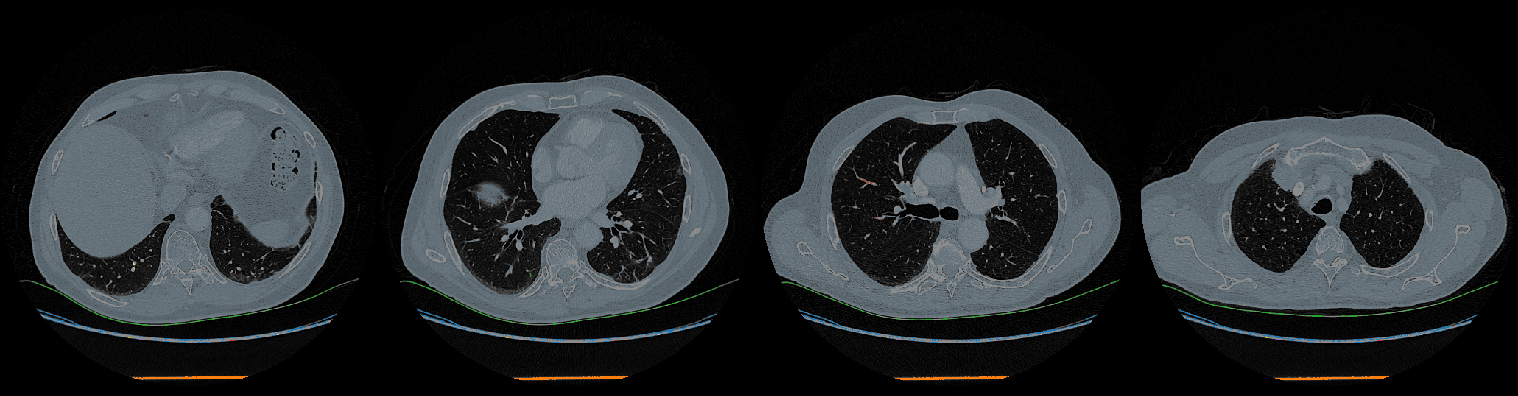
\includegraphics[width=\textwidth]{banner.png}\\[3pt]
  {\small\itshape Connected components of a CT soft-tissue mask, labelled by the \ufccl{} package (axial slices of one MSD Task06\_Lung scan).}
\end{center}
\vspace{10pt}
{\large\textbf{Subject:} \SubjectName}\par
\vspace{4pt}
{\large\textbf{Submitted By:}}\par
\vspace{2pt}
\begin{tabular}{@{}p{6.4cm}p{3.2cm}p{4.6cm}@{}}
  \toprule
  \rowcolor{sitlight}\textbf{Name} & \textbf{Branch} & \textbf{PRN}\\
  \midrule
  \AuthorOne & \BranchOne & \PRNOne\\
  \AuthorTwo & \BranchTwo & \PRNTwo\\
  \bottomrule
\end{tabular}
\par\vspace{8pt}
{\large\textbf{Under the guidance of:} \GuideName}\par
{\large\textbf{Submitted:} \ReportDate}
\clearpage

% =====================================================================
%  INDEX
% =====================================================================
\FrontHeading{INDEX}
{\small\printtoc}
\vspace{10pt}
\begin{center}\small\itshape
  The software, test suite, raw benchmark data and all figures of this report are in the project repository\\ (\texttt{ufccl3d/} and \texttt{report/}); Appendix~A lists the commands that reproduce every number.
\end{center}
\clearpage

% =====================================================================
%  ACKNOWLEDGEMENT
% =====================================================================
\phantomsection
\addcontentsline{toc}{section}{Acknowledgement}
\FrontHeading{ACKNOWLEDGEMENT}
We take this opportunity to express our heartfelt gratitude to everyone who has guided and supported us throughout the completion of our project titled \emph{``Union-Find Connected Component Labeling for Volumetric Medical Scans''}.

First and foremost, we extend our deepest thanks to \GuideName, our professor and project guide, for constant encouragement, valuable guidance and continuous support. Their insightful feedback and in-depth knowledge helped us understand the technical intricacies of disjoint-set data structures, memory-bounded algorithm design and rigorous experimental evaluation, and to turn a classical algorithm into a validated, benchmarked software package. Their mentorship has been a constant source of inspiration throughout this journey.

We would like to express our sincere gratitude to \DirectorName, Director of Symbiosis Institute of Technology, Hyderabad, for providing us with the necessary infrastructure, resources and an environment that encourages innovation, experimentation and research. Their vision for academic excellence has motivated us to pursue this project with dedication and care.

We are grateful to the Medical Segmentation Decathlon organisers and the contributing institutions for releasing de-identified CT data under an open licence, and to the authors and maintainers of the open-source tools on which this work rests: NumPy, SciPy, Numba, \texttt{cc3d}, nibabel, pydicom, Matplotlib and Hypothesis.

Finally, we would like to thank our peers and classmates for their helpful suggestions, cooperation and moral support, and Symbiosis Institute of Technology, Hyderabad, for providing the platform and resources to transform our ideas into reality.
\clearpage

% =====================================================================
%  ABSTRACT
% =====================================================================
\phantomsection
\addcontentsline{toc}{section}{Abstract}
\FrontHeading{ABSTRACT}
Connected component labeling (CCL) turns a binary segmentation of a volumetric scan into a list of separate regions, so that every lesion, nodule or vessel segment can be counted and measured. This project implements three-dimensional CCL with Union-Find (disjoint-set union with path halving and union by size) in Python and Numba, and extends the classical two-pass algorithm in three ways. \textbf{(i)}~Per-component statistics (voxel count, physical volume, centroid, bounding box) are accumulated in the same sweep that relabels the volume. \textbf{(ii)}~A \emph{slice-streaming} variant keeps only two slices of provisional labels and emits each lesion as soon as it ends, so its memory does not depend on the number of slices. \textbf{(iii)}~A \emph{tiled out-of-core} variant labels fixed-size tiles independently and joins them with a seam merge over a global Union-Find. All variants support 6-, 18- and 26-connectivity, and the in-memory and tiled label volumes are bit-identical to those of \texttt{scipy.ndimage.label}.

The implementation is validated by 130 automated tests (including property-based tests and dedicated seam tests) and by 390 oracle comparisons against SciPy and \texttt{cc3d}. It is benchmarked on synthetic volumes of up to $512^3$ voxels and on all 63 training CT scans of the Medical Segmentation Decathlon lung task (4.63 billion voxels). On CT soft-tissue masks the in-memory labeler is $1.7\times$ faster than SciPy and $2.1\times$ slower than \texttt{cc3d}; on the three largest scans the streaming variant needs 4--5~MB of working memory instead of 706--794~MB, and the tiled variant 26--36~MB. Counted Union-Find work per voxel stays flat from $3\times10^{4}$ to $1.7\times10^{7}$ voxels, matching the near-linear bound. This is a computational method evaluated on public and synthetic data; it is not a diagnostic tool.

\medskip
\textbf{Keywords:} connected component labeling, Union-Find, disjoint sets, 3-D medical imaging, streaming algorithms, out-of-core processing, lesion counting, CT.
\clearpage

% =====================================================================
%  1. INTRODUCTION
% =====================================================================
\section{Introduction}
\subsection{Motivation}
A segmentation model or a threshold applied to a CT or MRI volume produces a binary mask in which every foreground voxel is marked, but the mask does not say \emph{how many} separate structures it contains. Lesion count, the volume of each lesion and its position are the quantities that clinical and research workflows actually use, for example to describe disease burden or to follow a lesion over time. The step that converts a mask into separate, individually measurable objects is \emph{connected component labeling}: every maximal set of touching foreground voxels receives one integer identifier.

Modern CT volumes are large. A chest scan of $512\times512\times600$ voxels holds 157 million voxels, and a labeling that keeps a 4-byte label for every voxel needs hundreds of megabytes before any auxiliary structure is counted. Batch processing of hundreds of scans, or integration into a scanner or archive workflow, makes both time and memory relevant.

\subsection{Problem statement}
Given a binary volume $V\in\{0,1\}^{Z\times Y\times X}$, a connectivity rule $c\in\{6,18,26\}$ and voxel spacing $(s_z,s_y,s_x)$, compute (a)~a label volume $L$ in which two foreground voxels carry the same positive label if and only if they are connected under $c$, and background is $0$; and (b)~for every component its voxel count, physical volume $n\,s_z s_y s_x$, centroid and axis-aligned bounding box.

\subsection{Objectives and contributions}
The two-pass algorithm of Rosenfeld and Pfaltz~\cite{rosenfeld1966} and the analysis of Union-Find by Tarjan~\cite{tarjan1975} are classical, so the contribution of this project lies in the engineering and in the evaluation:
\begin{enumerate}
  \item An in-memory two-pass labeler with Union-Find, a tight bound on the number of provisional labels, and statistics fused into the relabeling sweep.
  \item A \textbf{slice-streaming} labeler that finalises each component as soon as it ends and never builds a label volume.
  \item A \textbf{tiled out-of-core} labeler with a seam merge, whose output is identical to the in-memory result.
  \item A \textbf{rigorous evaluation}: exact comparison with SciPy and \texttt{cc3d}, property-based and seam tests, operation counting for the Union-Find, scaling and peak-memory measurements, and a study on 63 public CT scans.
\end{enumerate}

\subsection{Organisation of the report}
Section~2 gives the background, Sections~3--5 the algorithms, their validation and the experimental set-up, Section~6 the results, and Sections~7--8 the limitations and conclusions. Appendix~A lists the commands that reproduce every number.

% =====================================================================
%  2. BACKGROUND
% =====================================================================
\section{Background and Related Work}
\subsection{Labeling by equivalence classes}
In a raster scan every voxel is compared only with neighbours that have already been visited. A voxel may touch two provisional labels that were created separately; those labels are then \emph{equivalent}. Recording such equivalences and resolving them afterwards is the two-pass scheme of~\cite{rosenfeld1966}. Union-Find (disjoint-set union)~\cite{galler1964} maintains the equivalence classes with two operations: $\textsc{find}(x)$ returns the representative of $x$'s set and $\textsc{union}(a,b)$ merges two sets. With union by size and path compression or halving, the amortised cost per operation is $O(\alpha(n))$, where $\alpha$ is the inverse Ackermann function~\cite{tarjan1975,tarjan1984}; for any practical $n$ it is at most 4. The total cost of labeling $N$ voxels is therefore $O(N\,\alpha(N))$.

\subsection{Connectivity in three dimensions}
Which voxels count as neighbours is a modelling choice. Table~\ref{tab:conn} lists the three standard rules and Fig.~\ref{fig:causal} shows the causal neighbours, those visited before the current voxel in $(z,y,x)$ raster order.

\begin{table}[!t]
\centering
\caption{Three-dimensional connectivity rules.}\label{tab:conn}
\small
\begin{tabular}{@{}cccp{8.2cm}@{}}
\toprule
\hrow Rule & Neighbours & Causal & Contact types included\\
\midrule
6  & 6  & 3  & faces only; does not merge structures that touch diagonally\\
18 & 18 & 9  & faces and edges\\
26 & 26 & 13 & faces, edges and corners\\
\bottomrule
\end{tabular}
\end{table}

\begin{figure}[!t]
\centering
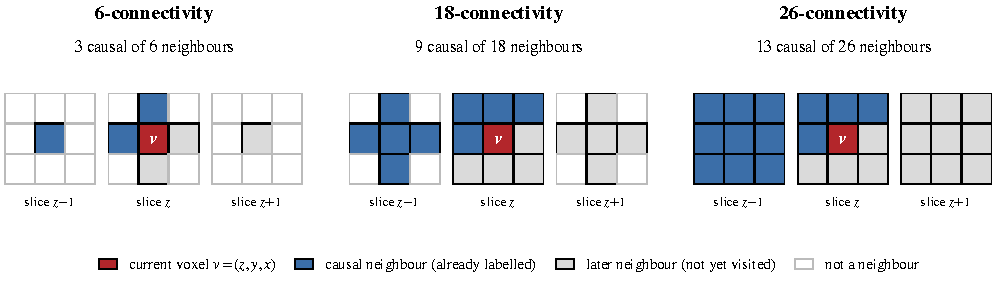
\includegraphics[width=0.95\textwidth]{figures/fig_causal.pdf}
\caption{Causal neighbourhoods used by the scan for 6-, 18- and 26-connectivity. Each group shows the three slices $z{-}1$, $z$ and $z{+}1$ around the current voxel~$v$; blue cells have already been labelled when $v$ is reached.}\label{fig:causal}
\end{figure}

For lesion work, 6-connectivity is the usual default because it does not join two lesions through a diagonal contact. The choice matters in practice: on the tumour annotations of the 63 CT scans used later, 6-connectivity gives 164 components, 18-connectivity 144 and 26-connectivity 141 (Fig.~\ref{fig:reallesions}c). The connectivity is therefore always stated explicitly in this report.

\subsection{Related work}
Run-based two-scan labeling~\cite{he2008} and block-based labeling with decision trees~\cite{grana2010} reduce the number of neighbour checks and Union-Find operations in 2-D; Wu et al.~\cite{wu2009} study optimisations of two-pass algorithms in general. In practice, 3-D labeling is available in SciPy (\texttt{scipy.ndimage.label})~\cite{scipy2020}, in ITK, and in the highly optimised \texttt{cc3d} library~\cite{cc3d}. These tools label a volume held entirely in memory. The present work does not compete with them on raw speed; it adds the streaming and tiled variants and the fused statistics, and it measures their cost against these tools under identical conditions.

% =====================================================================
%  3. METHODOLOGY
% =====================================================================
\section{Methodology}
\subsection{Two-pass labeling with Union-Find}
Algorithm listing~\ref{lst:twopass} summarises the in-memory labeler. Pass~1 assigns provisional labels in raster order and records equivalences; pass~2 resolves every provisional label to its root, numbers the roots consecutively and rewrites the volume in place.

\begin{lstlisting}[caption={Two-pass labeling (6-connectivity shown; 18 and 26 extend the causal set).},label={lst:twopass},float=t,captionpos=b,belowcaptionskip=2pt]
pass 1:  for z, y, x in raster order:
             if mask[z,y,x] == 0: continue
             nb = nonzero labels among lab[z-1,y,x], lab[z,y-1,x], lab[z,y,x-1]
             if nb is empty:   next_id += 1;  lab[z,y,x] = next_id
             else:             m = min(nb);   lab[z,y,x] = m
                               for v in nb:   if v != m: union(m, v)
pass 2:  for i in 1..next_id:  r = find(i);  if root_final[r] == 0: root_final[r] = ++n
                               final[i] = root_final[r]
         for each voxel:       lab[z,y,x] = final[lab[z,y,x]]       (in place)
\end{lstlisting}

Four implementation details matter for correctness and memory.
\begin{itemize}
  \item \textbf{Separate maps.} The map from root to final id (\texttt{root\_final}) is distinct from the map from provisional id to final id (\texttt{final}); sharing one array would overwrite a root's entry while other provisional ids still refer to it.
  \item \textbf{Tight label bound.} Every provisional label is created at the start of a foreground run along $x$, so the number of run starts bounds the number of labels. One cheap sweep computes it, and the Union-Find arrays are sized to it instead of to $N/2$; the bound is $N/2$ only for a checkerboard.
  \item \textbf{In-place relabeling.} The label volume is rewritten in place, so only one $4N$-byte array is needed for 32-bit labels.
  \item \textbf{Deterministic numbering.} Because provisional ids are created in raster order, final ids follow the order of first appearance, the same numbering as \texttt{scipy.ndimage.label}.
\end{itemize}

\subsection{Statistics fused into the relabeling sweep}
Each component owns a row of 11 integers: voxel count, the sums of $z$, $y$, $x$, the minimum and maximum of each coordinate, and the smallest raster index of any of its voxels. Two rows merge by adding the count and sums and taking minima and maxima, so a row can be folded into the row of its Union-Find root at any time. In the in-memory labeler the rows are filled during pass~2, in the same sweep that writes the final labels, so no extra read of the volume is needed. Centroid, bounding box and physical volume $n\,s_zs_ys_x$ follow directly from a row; the smallest raster index reproduces the first-appearance order.

\subsection{Slice-streaming labeling}
Only the previous and the current slice of labels are kept (Fig.~\ref{fig:streaming}a). Labels $1..K$ are the components touching the previous slice (the \emph{frontier}), and labels $K{+}1..M$ are created in the current slice. For 6-connectivity, $K$ and the number of new labels are each at most $\lceil YX/2\rceil$, because components that coexist in one slice cannot touch, so one representative voxel per component forms an independent set of the 2-D grid. After a slice is scanned, every non-root stats row is folded into its root, and each root is classified: a root carried by no voxel of the current slice is \emph{closed}, its row is emitted and its slot freed; every other root stays open, is renumbered $1..K'$ by an order-preserving in-place compaction, and the current labels are remapped to become the next frontier.

\textit{Why closing is safe.} A voxel of a later slice can only be adjacent to voxels of the slice directly before it. If no voxel of a component lies in slice $z$, no voxel of any slice after $z$ can ever join it. This is the zero reference-count condition; the per-slice remap pass recounts the frontier voxels per root, which the renumbering needs anyway. Working arrays grow adaptively from the run-start bound of each slice, so for sparse masks they stay small. Peak memory is $O(YX+\text{open components})$ plus the output table, independent of~$Z$.

\begin{figure}[!t]
\centering
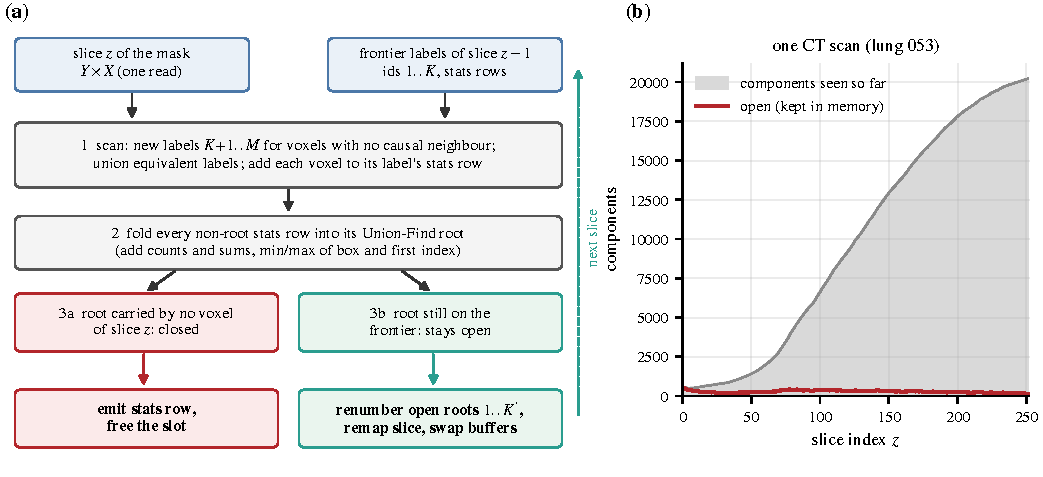
\includegraphics[width=0.95\textwidth]{figures/fig_streaming.pdf}
\caption{(a)~Processing of one slice by the streaming labeler. (b)~Components held in memory for one real CT soft-tissue mask (MSD scan lung\_053, 252 slices): at most 574 components are open at any time, whereas 20\,208 components are found in total.}\label{fig:streaming}
\end{figure}

\subsection{Tiled out-of-core labeling}
For volumes that do not fit in memory the volume is cut into tiles (128$^3$ by default), processed as follows (Fig.~\ref{fig:tiled}).
\begin{enumerate}
  \item Each tile is read, labeled independently and written back with \emph{global provisional ids} (tile offset plus local id); per-tile stats rows are kept.
  \item \textbf{Seam merge.} For each tile the tile plus a one-voxel halo is read. Every boundary voxel is compared with its causal neighbours that lie outside the tile (across faces, edges and corners, as the connectivity requires), and the pair of labels is united in a global Union-Find. Each adjacent voxel pair is examined exactly once, from the tile of its later voxel, and the high-side halo is needed for offsets such as $(-1,+1,0)$.
  \item Roots are numbered by their smallest raster index, stats rows are folded into roots, and every tile is rewritten with final ids.
\end{enumerate}
Because the numbering is by smallest raster index, the tiled output equals the in-memory output exactly. Labels and masks are read and written with explicit file I/O, so only one tile and the global Union-Find (one entry per tile-local component) are resident.

\begin{figure}[!t]
\centering
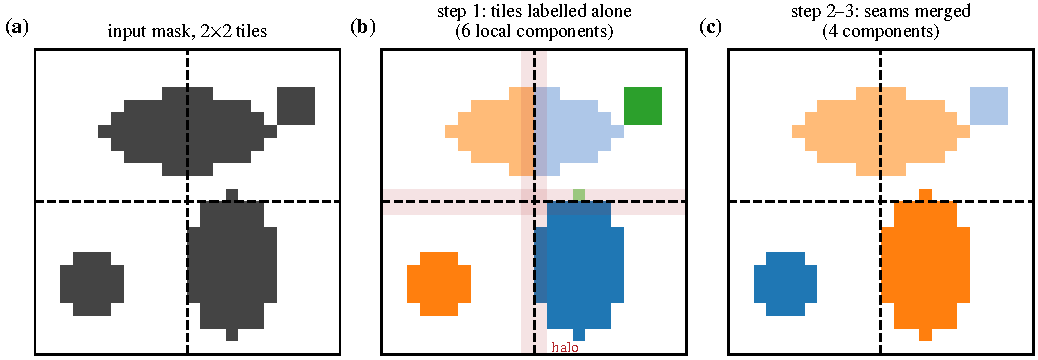
\includegraphics[width=0.95\textwidth]{figures/fig_tiled.pdf}
\caption{Tiled labeling on a small 2-D example (the 3-D code is identical in structure). (a)~Input mask cut into $2\times2$ tiles. (b)~Tiles labeled independently give 6 local components; the shaded band is the halo read for the seam merge. (c)~After the merge, 4 components remain.}\label{fig:tiled}
\end{figure}

\subsection{Complexity summary}
Table~\ref{tab:variants} compares the three variants. All three perform the same Union-Find work; they differ in what is kept in memory and in what is produced.

\begin{table}[!t]
\centering
\caption{Time, working memory and output of the three variants ($N$ voxels, slice size $YX$, $R$ foreground runs along $x$, tile edge $T$).}\label{tab:variants}
\small
\begin{tabular}{@{}lllp{4.6cm}@{}}
\toprule
\hrow Variant & Time & Working memory & Output\\
\midrule
In-memory & $O(N\,\alpha(N))$ & $N+4N+8R$ bytes & label volume + table\\
Streaming & $O(N\,\alpha(N))$ & $O(YX+\text{open})$ + table & table only\\
Tiled & $O(N\,\alpha(N))$ & $O(T^3)$ + $O(\text{tile-local comps.})$ & label volume on disk + table\\
\bottomrule
\end{tabular}
\end{table}

% =====================================================================
%  4. IMPLEMENTATION AND VALIDATION
% =====================================================================
\section{Implementation and Validation}
\subsection{Software}
The package \ufccl{} (Python~3.10, NumPy, Numba~\cite{numba2015}) is organised by responsibility: \texttt{unionfind} (find, union, statistics rows), \texttt{label} (in-memory), \texttt{streaming}, \texttt{tiled}, \texttt{volume} (RAM and raw-file block access), \texttt{io} (NIfTI via nibabel with RAS+ reorientation and spacing; DICOM series via pydicom with rescale to Hounsfield units), \texttt{synth} (phantoms), \texttt{validate} (partition equivalence) and \texttt{instrumented} (operation counting). Inner loops are compiled with \texttt{@njit}; a separate specialised kernel handles 6-connectivity, and 18/26-connectivity use a generic causal-offset loop. An application, \texttt{apps/lesion\_count.py}, chains mask, labeling, size filter, per-lesion CSV and a figure.

\subsection{Validation strategy}
Correctness of CCL is well defined: two labelings are equivalent if they induce the same partition of the foreground. The test suite (130 tests) checks this at several levels.
\begin{itemize}
  \item \textbf{Union-Find:} random operation sequences against a naive set model; union-by-size and path-halving properties; stats-row merging.
  \item \textbf{Oracles:} exact equality with \texttt{scipy.ndimage.label} (6, 18, 26) and partition equality with \texttt{cc3d}; centroid, bounding box and first index against SciPy measurements.
  \item \textbf{Degenerate inputs:} empty, full, single voxel, single line, checkerboard (maximum label count), serpentine path, volumes with a unit dimension, non-boolean dtypes.
  \item \textbf{Property-based (Hypothesis):} random volumes up to $9^3$ with random tile sizes down to a single voxel; streaming and tiled results must equal the in-memory result.
  \item \textbf{Seams:} lines crossing every seam along each axis; edge and corner contacts across tile boundaries, including the high-side case; file-backed out-of-core runs.
\end{itemize}
To check that the seam tests have teeth, the high-side halo was temporarily removed from the seam merge: six tests failed, and all passed again after the change was reverted.

% =====================================================================
%  5. EXPERIMENTAL SET-UP
% =====================================================================
\section{Experimental Set-up}
\textbf{Hardware and software.} AMD Ryzen~5 5600H (6 cores, used single-threaded), 15.4~GB RAM, Windows~11; Python~3.10.11, NumPy~2.2.6~\cite{numpy2020}, Numba~0.67, SciPy~1.15.3, \texttt{cc3d}~4.1.1. Timings are the best of 3--5 runs after JIT warm-up.

\textbf{Baselines.} \texttt{scipy.ndimage.label} and \texttt{cc3d.connected\_components}, both with the same connectivity.

\textbf{Synthetic data.} Three volume families give controlled structure (Fig.~\ref{fig:phantoms}): \emph{blobs} (thresholded, two-octave value noise; about 21\,\% foreground), \emph{lesions} (random ellipsoids and random-walk vessels; about 2.5\,\%) and \emph{noise} (independent voxels with $p=0.31$, close to the 6-connected site-percolation threshold~\cite{stauffer1994}, the hardest case with 7.2 million components at $512^3$).

\begin{figure}[!t]
\centering
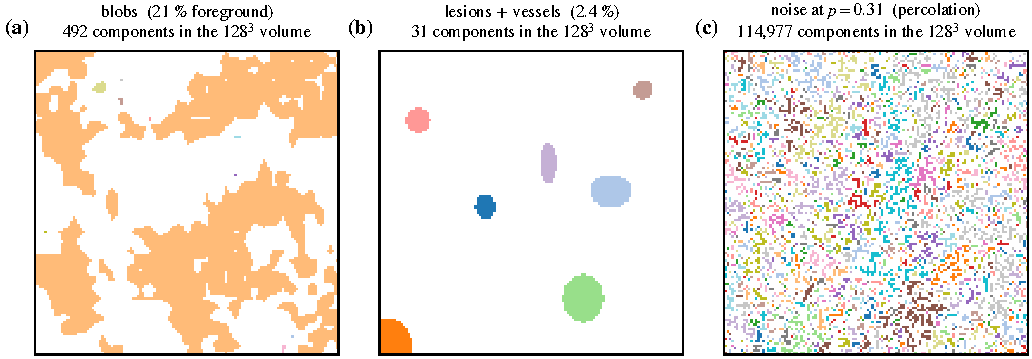
\includegraphics[width=0.95\textwidth]{figures/fig_phantoms.pdf}
\caption{Central slices of the three synthetic families ($128^3$ volumes), coloured by component label.}\label{fig:phantoms}
\end{figure}

\textbf{Real data.} All 63 training CT scans of the Medical Segmentation Decathlon lung task (Task06\_Lung; CC-BY-SA~4.0)~\cite{antonelli2022,simpson2019}: 112 to 636 slices of $512\times512$, 4.63 billion voxels in total. Two masks per scan are used: the \emph{tumour annotation} (label~1) and a \emph{soft-tissue window} of $[-200,300]$~HU. Volumes are reoriented to RAS+ and spacing is read from the NIfTI header.

\textbf{Metrics.} Exactness (array equality with SciPy), wall-clock time and throughput, peak extra working set measured in a separate process sampled every 3~ms after warm-up, and Union-Find operation counts (pointer steps per \textsc{find}).

% =====================================================================
%  6. RESULTS
% =====================================================================
\section{Results and Discussion}
\subsection{Correctness}
Table~\ref{tab:correct} summarises 130 volumes (random masks of varying shape and density, a checkerboard, a serpentine path, lesion phantoms, blobs and noise) at the three connectivities, 390 comparisons covering 76\,770 components. Every check passed. On the real data the exactness checks (SciPy, \texttt{cc3d}, streaming table, tiled output) passed for both masks at all three connectivities on 63 of 63 scans.

\begin{table}[!t]
\centering
\caption{Correctness checks on 130 volumes $\times$ 3 connectivities.}\label{tab:correct}
\small
\begin{tabular}{@{}lc@{}}
\toprule
\hrow Check & Passed\\
\midrule
Exact label-array equality with \texttt{scipy.ndimage.label} & 390/390\\
Partition equality with \texttt{cc3d} & 390/390\\
Streaming table equals in-memory table & 390/390\\
Tiled output equals in-memory output (random tiles of 1--19 voxels) & 390/390\\
Voxel counts and centroids equal SciPy's & 390/390\\
\bottomrule
\end{tabular}
\end{table}

\subsection{Speed}
Time grows linearly with $N$ for every method from $64^3$ to $512^3$ (Fig.~\ref{fig:scaling}). Table~\ref{tab:time} gives the $512^3$ case. For volumes of $256^3$ voxels and larger the in-memory labeler is $1.3$--$2.5\times$ faster than SciPy (smallest gain on noise, largest on sparse lesions) and $1.3$--$1.7\times$ slower than \texttt{cc3d}. Throughput is highest on sparse masks (173~\Mvox{}) and lowest at the percolation threshold (49~\Mvox{}), where nearly every voxel creates or merges a label. Computing the statistics in the same sweep costs up to about 30\,\% extra, and less than a separate statistics pass over the finished label volume (on blobs at $512^3$: $+0.04$~s against 0.28~s).

\begin{figure}[!t]
\centering
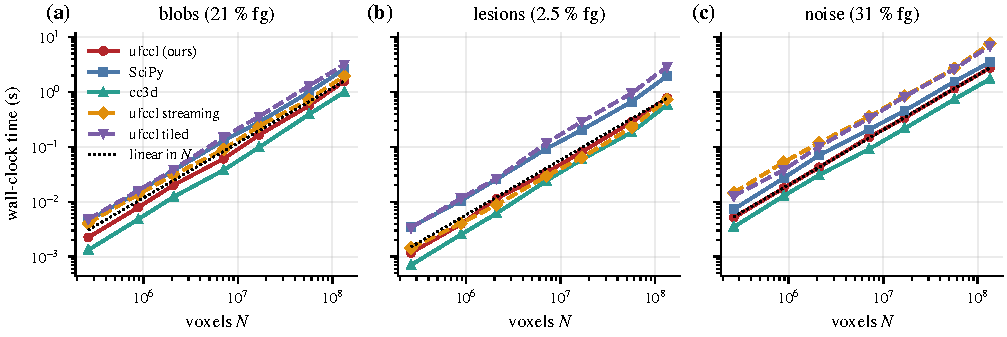
\includegraphics[width=0.95\textwidth]{figures/fig_scaling.pdf}
\caption{Wall-clock time against volume size for 6-connectivity (log--log). All methods are linear in the number of voxels.}\label{fig:scaling}
\end{figure}

\begin{table}[!t]
\centering
\caption{Time in seconds for $512^3$ volumes (134 million voxels), 6-connectivity, labels held in RAM.}\label{tab:time}
\small
\begin{tabular}{@{}lrrrrrrr@{}}
\toprule
\hrow Input & Components & \ufccl{} & + stats & SciPy & cc3d & Stream & Tiled\\
\midrule
blobs   & 32\,818 & 1.58 & 1.62 & 2.62 & \textbf{1.00} & 1.96 & 3.17\\
lesions & 1\,593 & 0.78 & 0.72 & 1.96 & \textbf{0.58} & 0.73 & 2.88\\
noise   & 7\,181\,695 & 2.73 & 3.58 & 3.48 & \textbf{1.72} & 7.51 & 6.87\\
\bottomrule
\end{tabular}
\end{table}

18- and 26-connectivity run the generic offset loop and are slower (Fig.~\ref{fig:speedconn}b): on blobs at $512^3$, 26-connectivity takes 4.3~s against 0.94~s for \texttt{cc3d}. No run-based scanning or decision trees were implemented, which is the main reason \texttt{cc3d} remains faster. The streaming variant is as fast as the in-memory one on sparse masks but 2.7 times slower on noise, where each slice emits and renumbers a large frontier.

\begin{figure}[!t]
\centering
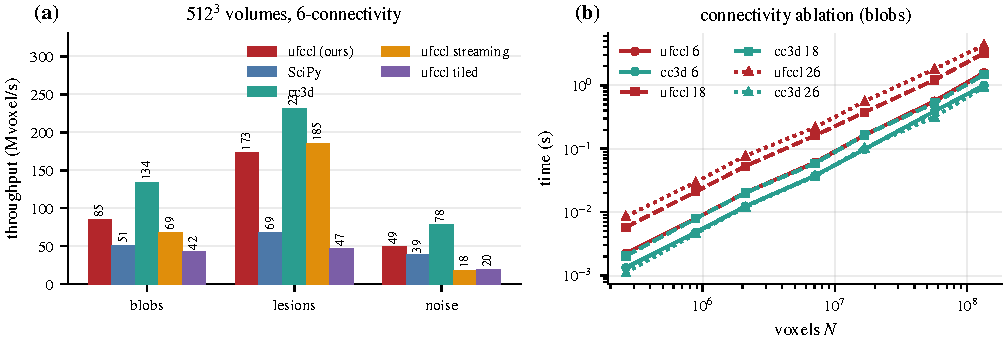
\includegraphics[width=0.95\textwidth]{figures/fig_speed_conn.pdf}
\caption{(a)~Throughput at $512^3$ for 6-connectivity. (b)~Effect of connectivity on the blob volumes.}\label{fig:speedconn}
\end{figure}

\subsection{Memory}
Peak working-set memory was measured in a separate process per run (Table~\ref{tab:mem}, Fig.~\ref{fig:memory}). At $512^3$ the in-memory labeler needs 662~MB (the input mask plus 4 bytes per voxel), SciPy 644~MB and \texttt{cc3d} 900~MB. The tiled variant, with masks and labels on disk, needs 43~MB, and the streaming variant 9.6~MB, about 69 times less than in memory. With the slice size fixed at $256\times256$ the in-memory labeler grows linearly with depth (40, 161 and 662~MB for 128, 512 and 2048 slices) while streaming stays at 1.2, 1.8 and 4.1~MB. At 8192 slices it rises to 36~MB; this growth is the output table (133\,220 components, 88 bytes each, copied a few times), not working state.

\begin{table}[!t]
\centering
\caption{Peak extra memory in MB over a post-warm-up baseline (blobs).}\label{tab:mem}
\small
\begin{tabular}{@{}lrrrrrr@{}}
\toprule
\hrow Volume & \ufccl{} & + stats & SciPy & cc3d & Tiled & Streaming\\
\midrule
$128^3$ & 9 & 10 & 10 & 13 & 33 & $<$1\\
$256^3$ & 80 & 83 & 81 & 112 & 34 & 1\\
$384^3$ & 273 & 274 & 271 & 380 & 37 & 4\\
$512^3$ & 662 & 663 & 644 & 900 & 43 & 10\\
\bottomrule
\end{tabular}
\end{table}

\begin{figure}[!t]
\centering
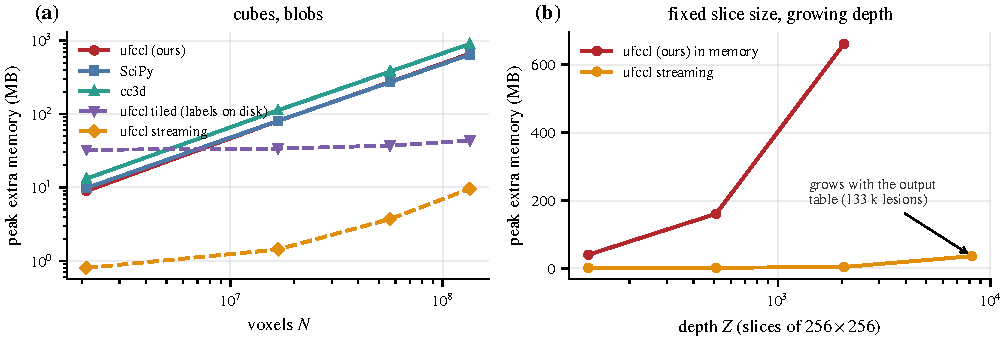
\includegraphics[width=0.95\textwidth]{figures/fig_memory.pdf}
\caption{Peak memory. (a)~Cubic volumes. (b)~Fixed $256\times256$ slices with growing depth.}\label{fig:memory}
\end{figure}

\subsection{Union-Find behaviour}
An instrumented kernel counts parent-pointer steps. With path halving and union by size, the number of steps per \textsc{find} stays between 0.4 and 0.95 and the longest single \textsc{find} is two steps on blob and noise volumes up to 16.8 million voxels (Fig.~\ref{fig:uf}a); the total work per voxel is flat in $N$, which is the measured counterpart of the $O(N\alpha(N))$ bound. The serpentine path proposed as a worst case is \emph{not} one for this scan order (longest \textsc{find}: 1). An adversarial \emph{comb} (many thin teeth that a final bar merges one by one) is: without compression and with naive linking the longest \textsc{find} is $W/2$ and the work grows quadratically (1\,333 steps per voxel at 48\,003 voxels), whereas halving with union by size stays at 0.17 steps per voxel for every size tested (Fig.~\ref{fig:uf}b). On realistic masks the variants differ little (Fig.~\ref{fig:uf}c): only the combination of no compression and naive linking is clearly bad (about 32 million steps against 122\,000 on blobs, 13 times slower).

\begin{figure}[!t]
\centering
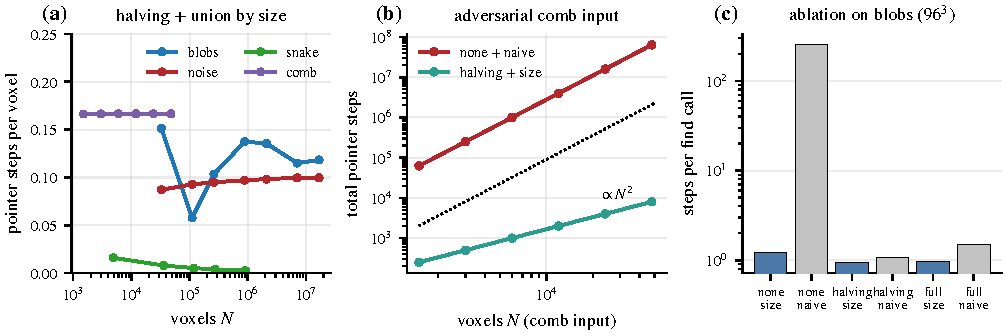
\includegraphics[width=0.95\textwidth]{figures/fig_uf.pdf}
\caption{Union-Find measurements. (a)~Pointer steps per voxel against $N$. (b)~Adversarial comb input. (c)~Ablation of compression (none, halving, full) and linking (union by size, naive) on a blob volume.}\label{fig:uf}
\end{figure}

\subsection{Real CT data: Medical Segmentation Decathlon lung task}
Fig.~\ref{fig:realct} shows one scan with 14 annotated tumour components, labeled by \ufccl{} and returned as a per-lesion table. For both masks and all three connectivities, SciPy (exact), \texttt{cc3d} (partition), the streaming table and the tiled output agreed with \ufccl{} on 63 of 63 scans. The soft-tissue masks contain 1.59 million components in total at 6-connectivity (0.45 million at 18, 0.33 million at 26).

\begin{figure}[!t]
\centering
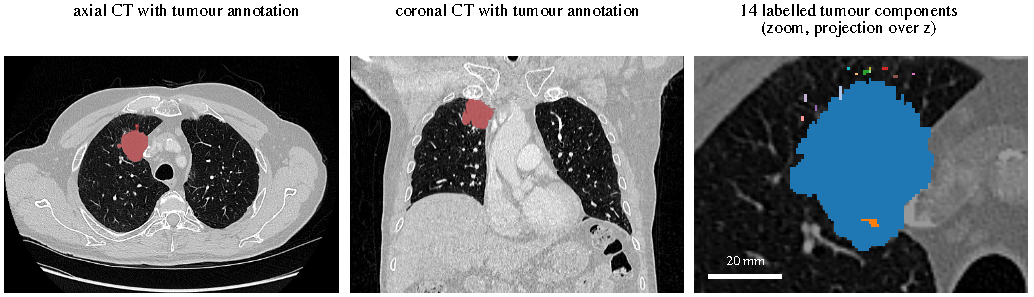
\includegraphics[width=0.95\textwidth]{figures/fig_real_ct.pdf}
\caption{MSD scan lung\_026 (RAS+, patient's right on the image left). (a,b)~Axial and coronal CT in a lung window with the tumour annotation in red. (c)~Zoom on the 14 labelled tumour components: one large mass and 13 small fragments, each with its own label.}\label{fig:realct}
\end{figure}

Table~\ref{tab:real} and Fig.~\ref{fig:realperf} give the cost over the 63 scans for the soft-tissue mask. Per scan, \ufccl{} is $1.72\times$ faster than SciPy (range 1.39--2.15) and $2.08\times$ slower than \texttt{cc3d} (1.70--2.53). On the very sparse tumour masks the total time over all scans is 12.2~s for \ufccl{}, 50.9~s for SciPy and 7.6~s for \texttt{cc3d}. On the three largest scans (149--167 million voxels) in-memory labeling needs 706--794~MB, \texttt{cc3d} 847--973~MB, the tiled variant 26--36~MB and the streaming variant 4--5~MB.

\begin{table}[!t]
\centering
\caption{Soft-tissue mask, 6-connectivity, 63 CT scans (4.63 G voxels): seconds per scan and total throughput.}\label{tab:real}
\small
\begin{tabular}{@{}lrrrr@{}}
\toprule
\hrow Method & Total (s) & Median (s) & Max (s) & \Mvox{}\\
\midrule
\ufccl{} & 38.2 & 0.56 & 1.32 & 121\\
\ufccl{} + stats & 48.2 & 0.71 & 1.74 & 96\\
SciPy & 65.8 & 0.97 & 2.33 & 70\\
cc3d & \textbf{18.2} & \textbf{0.28} & \textbf{0.61} & \textbf{254}\\
\ufccl{} streaming & 63.9 & 0.94 & 2.30 & 72\\
\ufccl{} tiled ($128^3$, RAM) & 100.1 & 1.47 & 3.57 & 46\\
\bottomrule
\end{tabular}
\end{table}

\begin{figure}[!t]
\centering
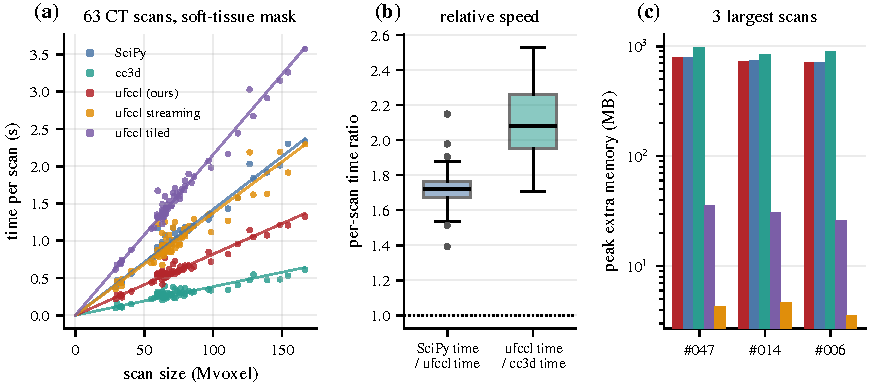
\includegraphics[width=0.95\textwidth]{figures/fig_real_perf.pdf}
\caption{Real CT, soft-tissue mask. (a)~Time per scan against scan size, with a line through the origin per method. (b)~Per-scan time ratios. (c)~Peak extra memory on the three largest scans (log scale; colours as in (a)).}\label{fig:realperf}
\end{figure}

The tumour annotations themselves contain 164 components at 6-connectivity, a median of one per scan (range 1--14). Their volumes are strongly skewed (Fig.~\ref{fig:reallesions}a): the median is 3~mm$^3$, 92 of the 164 components are smaller than 10~mm$^3$ (annotation fragments down to a single voxel), and the largest is 338~cm$^3$. A minimum-volume filter of 1000~mm$^3$ keeps 60 components and removes every component of three scans, so a fixed size threshold changes which scans count as having a lesion (Fig.~\ref{fig:reallesions}b). These annotations are the ground truth, so no detection or false-positive rate can be measured on them.

\begin{figure}[!t]
\centering
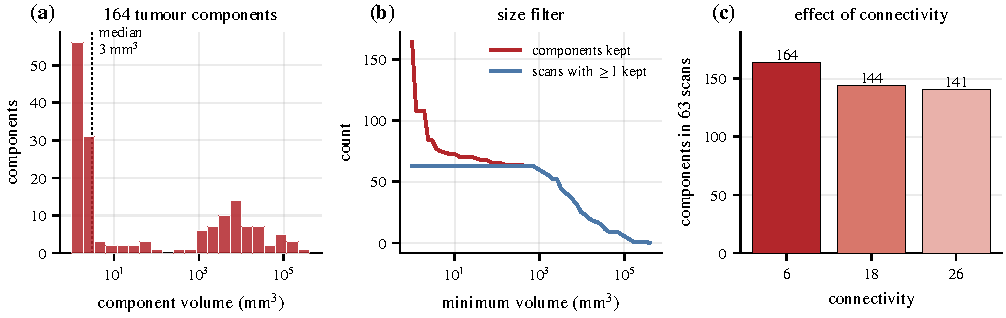
\includegraphics[width=0.95\textwidth]{figures/fig_real_lesions.pdf}
\caption{Tumour components of the 63 scans. (a)~Volume histogram (log scale). (b)~Components and scans kept as the minimum volume grows. (c)~Components found by each connectivity rule.}\label{fig:reallesions}
\end{figure}

\subsection{Lesion-counting application}
The application chains mask, labeling, size filter, per-lesion table and figure. To exercise it with a known reference, ten synthetic phantom scans ($96\times192\times192$ voxels, spacing $2.5\times0.8\times0.8$~mm) were combined with a simulated segmentation output (ragged boundaries, 10\,\% of lesions missed, 25 spurious blobs and speckle; voxel Dice 0.85). Without filtering the output has 742 components per scan, of which 726 are false positives. A size filter removes them: 24.8, 15.7, 4.5 and 0 false positives per scan at 5, 40, 80 and 160~mm$^3$, with lesion-wise sensitivity 0.927 without filtering and 0.893 with any filter. The false-positive sizes are set by the simulation, so this demonstrates the pipeline and not the behaviour of a real model.

% =====================================================================
%  7. LIMITATIONS
% =====================================================================
\section{Discussion and Limitations}
\textbf{Where each variant fits.} The in-memory labeler is the choice when the volume and its labels fit in memory and a label volume is needed. The streaming labeler is the choice when only the per-lesion table is needed, since it uses a few megabytes regardless of depth. The tiled labeler is the choice when a full label volume is needed but does not fit in memory. All three give the same components.

\textbf{Speed.} \texttt{cc3d} is faster on every input: $1.3$--$1.7\times$ on synthetic volumes of $256^3$ voxels and larger and $2.1\times$ on the CT soft-tissue masks. The case for \ufccl{} is memory-bounded operation with fused statistics, not raw speed. Run-based scanning and decision-tree neighbour checks~\cite{he2008,grana2010} are the natural next optimisations.

\textbf{Limits of the evidence.} Real data come from a single dataset (MSD Task06\_Lung, CT, 63 scans). No liver, vessel, LiTS, LIDC-IDRI or BraTS data were used, and no model predictions were available, so lesion-wise sensitivity and false positives are measured only on the synthetic study. Memory is sampled every 3~ms from the child process, so very short spikes could be missed. The code is single-threaded; no GPU or multi-process tiling was attempted. The streaming and tiled memory figures exclude the output table, which grows with the number of components. Tiled labels without statistics are numbered in tile order, not raster order.

\textbf{Clinical note.} This is a computational method evaluated on public and synthetic data. It is not a diagnostic tool and has not been validated for any clinical use.

% =====================================================================
%  8. CONCLUSION
% =====================================================================
\section{Conclusion and Future Work}
We implemented three-dimensional connected component labeling with Union-Find in three variants (in-memory, slice-streaming and tiled out-of-core), with per-lesion statistics fused into the labeling. All variants agree exactly with SciPy and \texttt{cc3d} on 130 test volumes and on 63 real CT scans at 6-, 18- and 26-connectivity, and the test suite includes seam and property-based tests. Time is linear in the number of voxels, the Union-Find does a measured constant amount of work per voxel, and on the largest CT scans streaming reduces working memory from about 750~MB to 4--5~MB and tiling to 26--36~MB. The in-memory labeler is $1.7\times$ faster than SciPy but $2.1\times$ slower than \texttt{cc3d} on the CT masks.

\textbf{Future work.} (1)~Run-based scanning and decision trees for the 6- and 26-connectivity kernels. (2)~Thread-level parallelism over tiles, which are independent until the seam merge, and a GPU kernel. (3)~Evaluation on further public data (liver and vessel tasks, LiTS, LIDC-IDRI, BraTS) and on predictions of a real segmentation model. (4)~A bounded-memory output path for the streaming table, and integration into an archive-style pipeline.

% =====================================================================
%  REFERENCES
% =====================================================================
\phantomsection
\addcontentsline{toc}{section}{References}
\begin{thebibliography}{99}\small
\setlength{\itemsep}{1pt}\setlength{\parskip}{0pt}
\bibitem{rosenfeld1966} A.~Rosenfeld and J.~L.~Pfaltz, ``Sequential operations in digital picture processing,'' \emph{J.\ ACM}, vol.~13, no.~4, pp.~471--494, 1966.
\bibitem{galler1964} B.~A.~Galler and M.~J.~Fischer, ``An improved equivalence algorithm,'' \emph{Commun.\ ACM}, vol.~7, no.~5, pp.~301--303, 1964.
\bibitem{tarjan1975} R.~E.~Tarjan, ``Efficiency of a good but not linear set union algorithm,'' \emph{J.\ ACM}, vol.~22, no.~2, pp.~215--225, 1975.
\bibitem{tarjan1984} R.~E.~Tarjan and J.~van Leeuwen, ``Worst-case analysis of set union algorithms,'' \emph{J.\ ACM}, vol.~31, no.~2, pp.~245--281, 1984.
\bibitem{he2008} L.~He, Y.~Chao and K.~Suzuki, ``A run-based two-scan labeling algorithm,'' \emph{IEEE Trans.\ Image Process.}, vol.~17, no.~5, pp.~749--756, 2008.
\bibitem{wu2009} K.~Wu, E.~Otoo and K.~Suzuki, ``Optimizing two-pass connected-component labeling algorithms,'' \emph{Pattern Anal.\ Appl.}, vol.~12, pp.~117--135, 2009.
\bibitem{grana2010} C.~Grana, D.~Borghesani and R.~Cucchiara, ``Optimized block-based connected components labeling with decision trees,'' \emph{IEEE Trans.\ Image Process.}, vol.~19, no.~6, pp.~1596--1609, 2010.
\bibitem{cc3d} W.~Silversmith, ``cc3d: connected components on multilabel 3D and 2D images,'' software, \url{https://github.com/seung-lab/connected-components-3d}.
\bibitem{scipy2020} P.~Virtanen \emph{et al.}, ``SciPy 1.0: fundamental algorithms for scientific computing in Python,'' \emph{Nat.\ Methods}, vol.~17, pp.~261--272, 2020.
\bibitem{numpy2020} C.~R.~Harris \emph{et al.}, ``Array programming with NumPy,'' \emph{Nature}, vol.~585, pp.~357--362, 2020.
\bibitem{numba2015} S.~K.~Lam, A.~Pitrou and S.~Seibert, ``Numba: a LLVM-based Python JIT compiler,'' in \emph{Proc.\ 2nd Workshop on the LLVM Compiler Infrastructure in HPC}, 2015.
\bibitem{antonelli2022} M.~Antonelli \emph{et al.}, ``The Medical Segmentation Decathlon,'' \emph{Nat.\ Commun.}, vol.~13, art.~4128, 2022.
\bibitem{simpson2019} A.~L.~Simpson \emph{et al.}, ``A large annotated medical image dataset for the development and evaluation of segmentation algorithms,'' arXiv:1902.09063, 2019.
\bibitem{stauffer1994} D.~Stauffer and A.~Aharony, \emph{Introduction to Percolation Theory}, 2nd ed., Taylor \& Francis, 1994.
\end{thebibliography}

% =====================================================================
%  APPENDIX
% =====================================================================
\clearpage
\appendix
\section*{Appendix A: Reproducing the Results}
\phantomsection
\addcontentsline{toc}{section}{Appendix A: Reproducing the Results}
The code is in \texttt{ufccl3d/} (package \texttt{ufccl/}, tests, \texttt{bench/}, \texttt{apps/}, \texttt{results/}); this report and its figure script are in \texttt{report/}.

\textbf{Commands.}
\begin{lstlisting}[numbers=none,frame=leftline,xleftmargin=6pt]
pip install numpy numba scipy nibabel pydicom matplotlib psutil pytest hypothesis \
            connected-components-3d
python -m pytest                                   # 130 tests
python bench/run_bench.py all                      # synthetic benchmarks
python bench/run_real.py PATH/Task06_Lung          # 63 real CT scans
python bench/plot_results.py                       # tables and plots
python -m apps.lesion_count --synthetic --out out/
python report/tools/make_figures.py PATH/Task06_Lung   # figures of this report
\end{lstlisting}

\textbf{Data.} Task06\_Lung was downloaded from the AWS Open Data registry for the Medical Segmentation Decathlon (\url{https://registry.opendata.aws/msd/}); only the training images and labels were used.

\end{document}
